\documentclass[12pt, a4paper]{article}

\usepackage[utf8]{inputenc}
\usepackage[T1]{fontenc}
\usepackage[polish]{babel}
\usepackage{geometry}
\usepackage{graphicx}
\usepackage{float}
\usepackage{booktabs}
\usepackage{array}
\usepackage{tabularx}
\usepackage{listings}
\usepackage{xcolor}
\usepackage{hyperref}
\usepackage{caption}
\usepackage{parskip}

\geometry{margin=2.5cm}

% SQL listing style
\lstdefinelanguage{SQL}{
  keywords={SELECT, FROM, WHERE, JOIN, ON, GROUP, BY, ORDER, INSERT, INTO,
            VALUES, CREATE, TABLE, PRIMARY, KEY, FOREIGN, REFERENCES,
            NOT, NULL, UNIQUE, DEFAULT, AS, ROUND, AVG, MAX, MIN, SUM,
            COUNT, DATE, LIMIT, AND, OR, IF, CONSTRAINT, SERIAL, INT,
            VARCHAR, NUMERIC, TIMESTAMP, TEXT, DO, NOTHING, CONFLICT, LEFT,
            COALESCE},
  keywordstyle=\color{blue}\bfseries,
  sensitive=false,
  comment=[l]{--},
  commentstyle=\color{gray}\itshape,
  stringstyle=\color{orange},
  morestring=[b]',
}

\lstset{
  language=SQL,
  basicstyle=\ttfamily\small,
  backgroundcolor=\color{gray!10},
  frame=single,
  breaklines=true,
  showstringspaces=false,
  tabsize=2,
}

\begin{document}

% ── Header table ─────────────────────────────────────────────────────────────

\begin{table}[H]
\centering
\begin{tabular}{|p{3cm}|p{3.5cm}|p{3.5cm}|p{3.5cm}|}
\hline
\textbf{Wydział:} & \textbf{Kierunek:} & \textbf{Przedmiot:} & \textbf{Skład zespołu:} \\
EAIIIB & Automatyka i Robotyka & Bazy danych & Otylia Rybak \\
       &             &             & Kamila Rebilas \\
       &             &             & Michał Rogowski \\
\hline
\textbf{Data oddania:} & \multicolumn{2}{l|}{\textbf{Temat:}} & \textbf{Raport końcowy} \\
Czerwiec 2026 & \multicolumn{2}{l|}{Baza danych i dashboard pogodowy} & \\
              & \multicolumn{2}{l|}{na podstawie Open-Meteo API} & \\
\hline
\end{tabular}
\end{table}

\vspace{0.5cm}

\noindent\textit{Źródło: Opracowanie własne na podstawie dokumentacji Open-Meteo API (\url{https://open-meteo.com/}).}

\noindent\textit{Środowisko uruchomienia: Python 3.13, PostgreSQL 18, Streamlit.}

\vspace{1cm}

% ── 1. Cel projektu ──────────────────────────────────────────────────────────

\section*{\textbf{1. Cel projektu}}

Celem projektu było zaprojektowanie i zaimplementowanie systemu do automatycznego
pobierania, przechowywania oraz wizualizacji danych pogodowych i jakości powietrza.
Dane pozyskiwano z darmowego Open-Meteo API dla dziewięciu wybranych lokalizacji
w Polsce i Europie. Wyniki importu zapisywano w relacyjnej bazie danych PostgreSQL,
a do ich prezentacji opracowano interaktywny dashboard w technologii Streamlit.

System realizuje trzy główne funkcje: cykliczne pobieranie prognoz pogodowych
i wskaźników jakości powietrza, ich trwałe przechowywanie z eliminacją duplikatów,
oraz wizualizację z możliwością filtrowania według wielu kryteriów. Projekt
podzielono na trzy części realizowane przez członków zespołu: warstwę importu danych,
schemat bazy danych z zapytaniami SQL oraz dashboard wraz z dokumentacją i raportem końcowym.

% ── 2. Wybór technologii ─────────────────────────────────────────────────────

\section*{\textbf{2. Wybór technologii}}

Przy doborze technologii kierowano się kryteriami dostępności, łatwości integracji
z bazą danych oraz możliwościami wizualizacyjnymi.

\textbf{Python 3.13} wybrano jako język implementacji ze względu na bogate
ekosystemowe wsparcie dla integracji z bazami danych (biblioteka SQLAlchemy),
przetwarzania danych tabelarycznych (pandas) oraz szybkiego tworzenia aplikacji
webowych. Do zarządzania zależnościami zastosowano menedżer \texttt{uv}, który
zapewnia szybką instalację pakietów i deterministyczne środowisko wirtualne
poprzez plik \texttt{uv.lock}.

\textbf{PostgreSQL 18} wybrano jako system zarządzania bazą danych ze względu na
pełne wsparcie relacyjnego modelu danych z kluczami obcymi, ograniczeniami
\texttt{UNIQUE} oraz klauzulą \texttt{ON CONFLICT}, która umożliwia
idempotentny zapis danych bez duplikatów. Alternatywą był SQLite, jednak brak
obsługi równoległych połączeń i ograniczone możliwości typów danych skłoniły
do wyboru PostgreSQL.

\textbf{Streamlit} wybrano do budowy dashboardu ze względu na możliwość tworzenia
interaktywnych aplikacji webowych wyłącznie w Pythonie, bez konieczności pisania
kodu HTML, CSS ani JavaScript. Biblioteka oferuje gotowe komponenty takie jak
suwaki, selectboxy, wykresy i kafelki metryczne, które bezpośrednio mapują się
na potrzeby projektu. W porównaniu do alternatyw takich jak Dash (Plotly) czy
Grafana, Streamlit wymaga znacznie mniej konfiguracji przy podobnych możliwościach
prezentacyjnych dla prototypu akademickiego.

\textbf{Open-Meteo API} wybrano ze względu na brak wymagań rejestracyjnych i brak
limitu zapytań dla użytku niekomercyjnego, co eliminuje konieczność zarządzania
kluczami API. Dane pogodowe opierają się na modelach meteorologicznych ECMWF
i DWD o wysokiej dokładności.

% ── 3. Opis API ──────────────────────────────────────────────────────────────

\section*{\textbf{3. Opis API}}

W projekcie wykorzystano trzy endpointy udostępniane przez Open-Meteo:

\begin{table}[H]
\centering
\begin{tabularx}{\textwidth}{|l|X|}
\hline
\textbf{Endpoint} & \textbf{Opis} \\
\hline
\texttt{api.open-meteo.com/v1/forecast} & Dane pogodowe godzinowe i dzienne: temperatura, wilgotność, opady, prędkość wiatru, kod pogody \\
\hline
\texttt{air-quality-api.open-meteo.com/v1/air-quality} & Dane jakości powietrza: PM2.5, PM10, europejski indeks AQI \\
\hline
\texttt{geocoding-api.open-meteo.com/v1/search} & Geokodowanie -- pobieranie współrzędnych geograficznych na podstawie nazwy miasta \\
\hline
\end{tabularx}
\caption{Tabela 1. Wykorzystane endpointy Open-Meteo API}
\end{table}

API nie wymaga klucza dostępu ani rejestracji. Dane zwracane są w formacie JSON
i obejmują prognozy na okres 3 dni z rozdzielczością godzinową. Kody pogodowe
zgodne są ze standardem WMO (World Meteorological Organization), co umożliwiło
stworzenie tabeli słownikowej z opisami słownymi stanów atmosferycznych.

Monitorowanymi lokalizacjami są: Kraków, Warszawa, Gdańsk, Wrocław, Zakopane,
Berlin, Paryż, Londyn oraz Rzym. Dobór lokalizacji obejmuje zarówno duże miasta
polskie, jak i europejskie stolice, co pozwala na porównanie warunków pogodowych
w różnych strefach klimatycznych.

% ── 4. Model bazy danych ─────────────────────────────────────────────────────

\section*{\textbf{4. Model bazy danych}}

Bazę danych zaprojektowano w PostgreSQL 18. Schemat składa się z czterech tabel
merytorycznych, jednej tabeli słownikowej oraz jednej tabeli technicznej do
rejestrowania historii importów.

\begin{table}[H]
\centering
\begin{tabularx}{\textwidth}{|l|X|}
\hline
\textbf{Tabela} & \textbf{Opis} \\
\hline
\texttt{locations} & Lokalizacje monitorowane przez system (miasto, szerokość i długość geograficzna) \\
\hline
\texttt{weather\_hourly} & Godzinowe dane pogodowe: temperatura, wilgotność, opady, prędkość wiatru, kod pogody \\
\hline
\texttt{weather\_daily} & Dzienne prognozy: temperatura min/max, wschód i zachód słońca \\
\hline
\texttt{air\_quality} & Godzinowe dane jakości powietrza: PM10, PM2.5, AQI \\
\hline
\texttt{dict\_weather\_code} & Słownik kodów WMO z opisami słownymi stanów pogody \\
\hline
\texttt{import\_log} & Logi importów: czas, status, liczba rekordów, komunikat błędu \\
\hline
\end{tabularx}
\caption{Tabela 2. Tabele w bazie danych}
\end{table}

Tabela \texttt{locations} pełni rolę centralną -- wszystkie tabele pomiarowe
odwołują się do niej kluczem obcym \texttt{location\_id}. Taka normalizacja
eliminuje redundancję nazw miast i współrzędnych geograficznych. Tabela
\texttt{dict\_weather\_code} przechowuje 28 opisów kodów WMO (np. kod 0 to
,,Czyste niebo'', kod 95 to ,,Burza'') i jest powiązana z \texttt{weather\_hourly}
przez \texttt{weather\_code}. Dzięki temu dashboard może wyświetlać opisy słowne
zamiast liczb, co widać na poniższym zrzucie:

\begin{figure}[H]
\centering
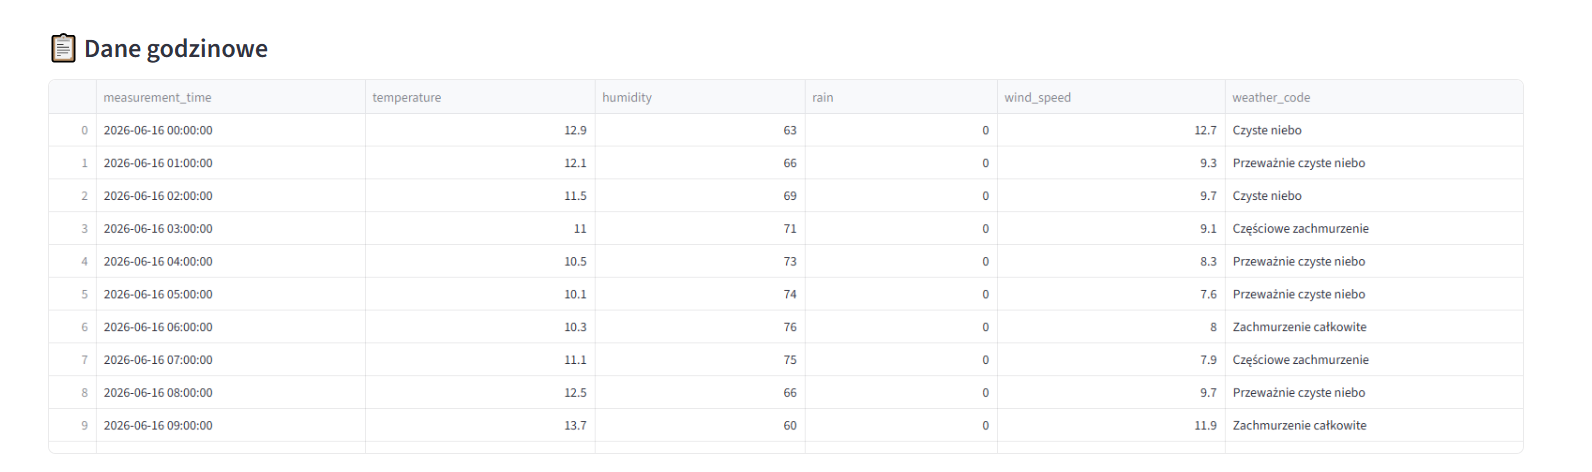
\includegraphics[width=0.95\textwidth]{img/tabela_godzinowa.png}
\captionof{figure}{Rysunek 1. Dane godzinowe z opisami kodów pogody}
\end{figure}

% ── 5. Diagram ERD ───────────────────────────────────────────────────────────

\section*{\textbf{5. Diagram ERD}}

\begin{figure}[H]
\centering
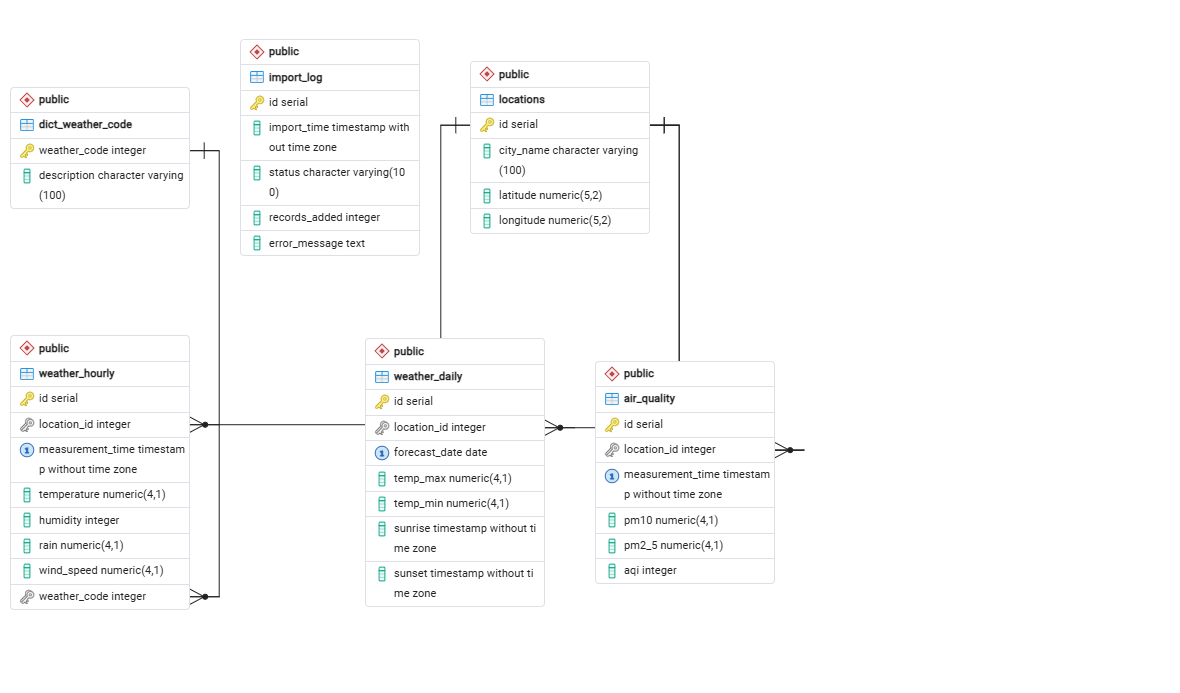
\includegraphics[width=0.95\textwidth]{img/erd.png}
\captionof{figure}{Rysunek 2. Diagram ERD bazy danych}
\end{figure}

Tabele \texttt{weather\_hourly}, \texttt{weather\_daily} oraz \texttt{air\_quality}
powiązane są kluczem obcym z tabelą \texttt{locations} (pole \texttt{location\_id}).
Tabela \texttt{weather\_hourly} powiązana jest dodatkowo z tabelą słownikową
\texttt{dict\_weather\_code} przez pole \texttt{weather\_code}.
Każda z tabel pomiarowych posiada ograniczenie \texttt{UNIQUE} na kombinacji
\texttt{location\_id} i czasu pomiaru, co zabezpiecza przed duplikatami
przy wielokrotnym uruchamianiu importu.

% ── 6. Opis importu danych ───────────────────────────────────────────────────

\section*{\textbf{6. Opis importu danych}}

Import danych zaimplementowano w pliku \texttt{api\_import.py} z użyciem
standardowej biblioteki \texttt{urllib} do komunikacji z API oraz \texttt{SQLAlchemy}
do zapisu w bazie danych. Połączenie z PostgreSQL realizowane jest przez sterownik
\texttt{psycopg2}. Proces importu przebiega w następujących etapach:

\begin{enumerate}
  \item Geokodowanie nazw miast z pliku konfiguracyjnego przy użyciu Geocoding API.
  \item Zapis lub aktualizacja współrzędnych lokalizacji w tabeli \texttt{locations}.
  \item Dla każdej lokalizacji: pobranie danych pogodowych (godzinowych i dziennych)
        oraz danych jakości powietrza.
  \item Zapis rekordów do odpowiednich tabel z użyciem klauzuli
        \texttt{ON CONFLICT DO UPDATE}, co eliminuje duplikaty.
  \item Zapis wpisu do tabeli \texttt{import\_log} ze statusem \texttt{SUCCESS}
        lub \texttt{FAILED} i liczbą dodanych rekordów.
\end{enumerate}

Import uruchamiany jest cyklicznie co 60 minut przez wbudowany scheduler.
Możliwe jest również jednorazowe uruchomienie przez parametr \texttt{-{}-once}
lub z niestandardowym interwałem przez \texttt{-{}-interval}. Przy pierwszym
uruchomieniu skrypt automatycznie tworzy bazę danych i wszystkie tabele,
co eliminuje konieczność ręcznej konfiguracji schematu.

% ── 7. Skrypty SQL ───────────────────────────────────────────────────────────

\section*{\textbf{7. Skrypty SQL}}

Przygotowano pliki \texttt{create\_tables.sql} oraz \texttt{insert\_initial\_data.sql}
umożliwiające odtworzenie bazy danych od zera bez uruchamiania skryptu Pythona.
Poniżej przedstawiono przykładową definicję tabeli \texttt{weather\_hourly}
ilustrującą zastosowanie kluczy obcych i ograniczenia unikalności:

\begin{lstlisting}
CREATE TABLE IF NOT EXISTS weather_hourly (
    id               SERIAL PRIMARY KEY,
    location_id      INT NOT NULL,
    measurement_time TIMESTAMP NOT NULL,
    temperature      NUMERIC(4, 1),
    humidity         INT,
    rain             NUMERIC(4, 1),
    wind_speed       NUMERIC(4, 1),
    weather_code     INT,
    CONSTRAINT fk_location
        FOREIGN KEY (location_id) REFERENCES locations(id),
    CONSTRAINT fk_weather_code
        FOREIGN KEY (weather_code)
        REFERENCES dict_weather_code(weather_code),
    CONSTRAINT unique_location_time
        UNIQUE (location_id, measurement_time)
);
\end{lstlisting}

% ── 8. Zapytania analityczne ─────────────────────────────────────────────────

\section*{\textbf{8. Zapytania analityczne SQL}}

Przygotowano pięć zapytań analitycznych zaimplementowanych w pliku \texttt{queries.py}.
Zapytania umożliwiają analizę danych bez użycia dashboardu -- mogą być
uruchamiane bezpośrednio z linii poleceń lub z poziomu narzędzia pgAdmin.

\textbf{Zapytanie 1 -- Aktualny przegląd pogody (ostatnie 24h):}
\begin{lstlisting}
SELECT l.city_name AS miasto,
       w.measurement_time AS data_godzina,
       w.temperature AS temperatura_c,
       w.humidity AS wilgotnosc_procent,
       w.wind_speed AS wiatr_kmh,
       d.description AS stan_pogody
FROM weather_hourly w
JOIN locations l ON w.location_id = l.id
JOIN dict_weather_code d ON w.weather_code = d.weather_code
ORDER BY w.measurement_time DESC
LIMIT 24;
\end{lstlisting}

\textbf{Zapytanie 2 -- Prognoza dzienna:}
\begin{lstlisting}
SELECT l.city_name AS miasto,
       wd.forecast_date AS data_prognozy,
       wd.temp_max AS maksymalna_temperatura,
       wd.temp_min AS minimalna_temperatura,
       wd.sunrise AS wschod_slonca,
       wd.sunset AS zachod_slonca
FROM weather_daily wd
JOIN locations l ON wd.location_id = l.id
ORDER BY wd.forecast_date ASC;
\end{lstlisting}

\textbf{Zapytanie 3 -- Alerty i anomalie pogodowe:}

Zapytanie wykrywa potencjalnie niebezpieczne warunki atmosferyczne: silny wiatr
(powyżej 25 km/h), temperaturę poniżej zera oraz kody pogodowe odpowiadające
intensywnym opadom deszczu (65, 82) i burzom (95, 99).

\begin{lstlisting}
SELECT l.city_name AS miasto,
       w.measurement_time AS czas_zdarzenia,
       w.temperature AS temperatura,
       w.wind_speed AS predkosc_wiatru,
       d.description AS zjawisko
FROM weather_hourly w
JOIN locations l ON w.location_id = l.id
JOIN dict_weather_code d ON w.weather_code = d.weather_code
WHERE w.wind_speed > 25.0
   OR w.temperature < 0.0
   OR w.weather_code IN (65, 82, 95, 99)
ORDER BY w.measurement_time DESC;
\end{lstlisting}

\textbf{Zapytanie 4 -- Średnie dobowe zanieczyszczenie powietrza:}
\begin{lstlisting}
SELECT l.city_name AS miasto,
       DATE(a.measurement_time) AS dzien,
       ROUND(AVG(a.pm10), 1) AS srednie_pm10,
       ROUND(AVG(a.pm2_5), 1) AS srednie_pm25,
       MAX(a.aqi) AS najwyzsze_aqi
FROM air_quality a
JOIN locations l ON a.location_id = l.id
GROUP BY l.city_name, DATE(a.measurement_time)
ORDER BY dzien DESC;
\end{lstlisting}

\textbf{Zapytanie 5 -- Statystyki techniczne systemu:}
\begin{lstlisting}
SELECT status,
       COUNT(*) AS liczba_uruchomien,
       SUM(records_added) AS lacznie_pobranych_rekordow
FROM import_log
GROUP BY status;
\end{lstlisting}

% ── 9. Dashboard ─────────────────────────────────────────────────────────────

\section*{\textbf{9. Opis dashboardu}}

Dashboard zaimplementowano przy użyciu biblioteki Streamlit w pliku
\texttt{dashboard/dashboard.py}. Połączenie z bazą danych nawiązywane jest
przez SQLAlchemy z użyciem dekoratora \texttt{@st.cache\_resource},
który zapewnia utrzymanie jednego połączenia przez całą sesję użytkownika.

Panel boczny zawiera 12 filtrów pogrupowanych tematycznie: wybór lokalizacji
i typu danych (godzinowe/dzienne/jakość powietrza), zakres dat i godzin,
progi temperaturowe z opcją wyświetlenia linii referencyjnych na wykresie,
maksymalne wartości opadu i wiatru, filtr kodu pogody oraz progi PM2.5, PM10
i AQI. Na górze strony wyświetlane są kafelki podsumowujące aktualne wartości.

\begin{figure}[H]
\centering
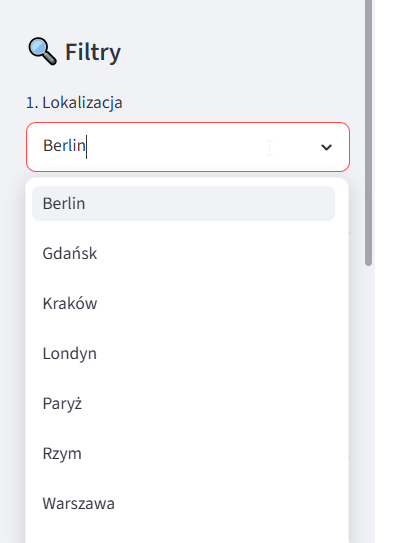
\includegraphics[width=0.35\textwidth]{img/dashboard_filtry.png}
\captionof{figure}{Rysunek 3. Panel filtrów dashboardu}
\end{figure}

\begin{figure}[H]
\centering
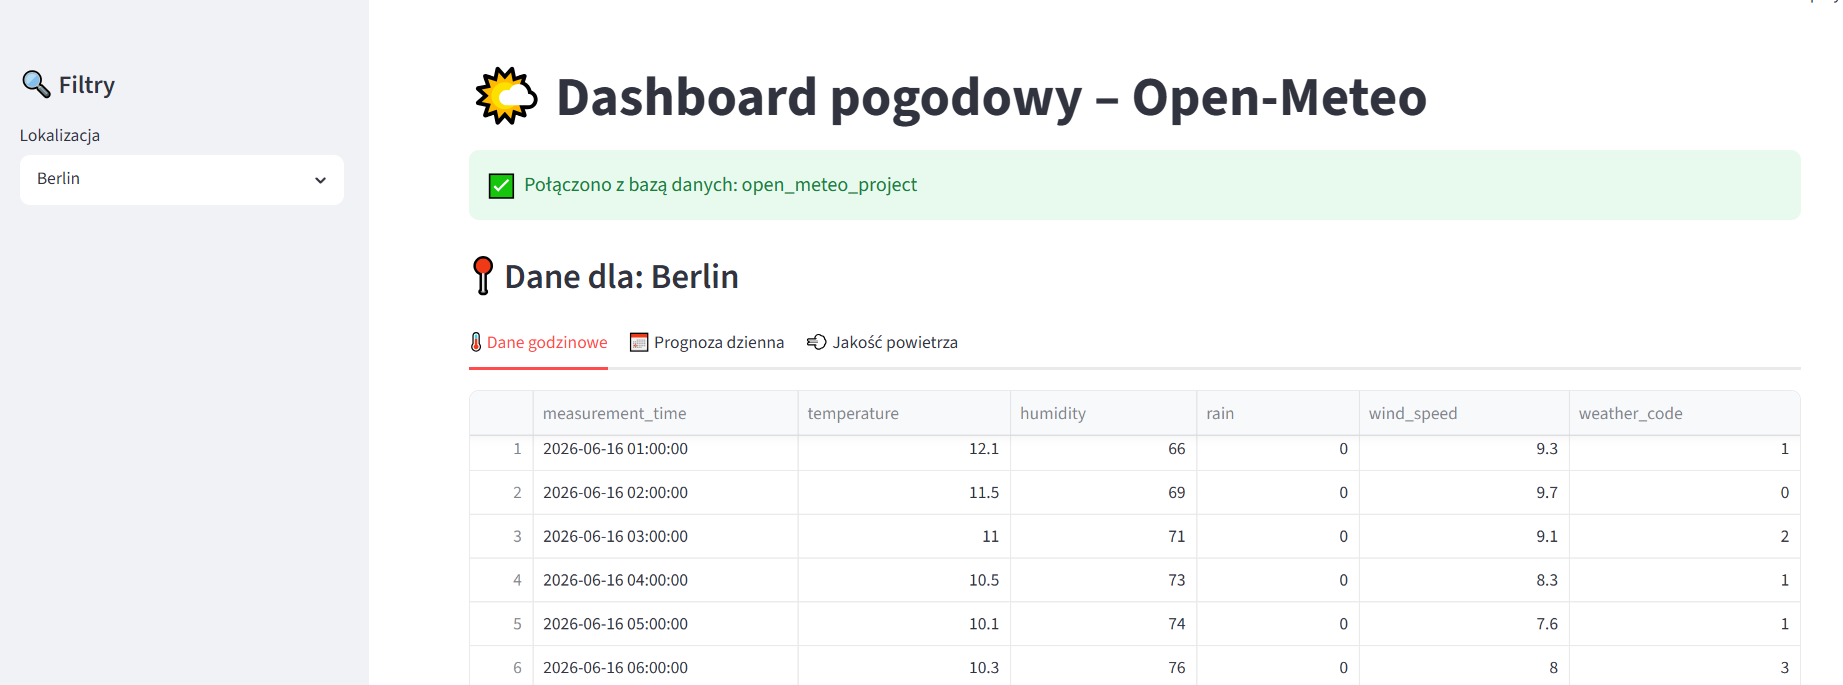
\includegraphics[width=0.95\textwidth]{img/dashboard_ogolny.png}
\captionof{figure}{Rysunek 4. Dashboard -- widok ogólny z tabelą danych godzinowych}
\end{figure}

Widok godzinowy prezentuje wykresy temperatury (liniowy), opadów (słupkowy)
oraz prędkości wiatru (liniowy z linią limitu). Dla wiatru linia limitu
jest zawsze widoczna -- pozwala to ocenić, czy zmierzone wartości przekraczają
ustawiony próg bez ukrywania danych. Dla temperatury linie limitów są opcjonalne
i domyślnie wyłączone.

\begin{figure}[H]
\centering
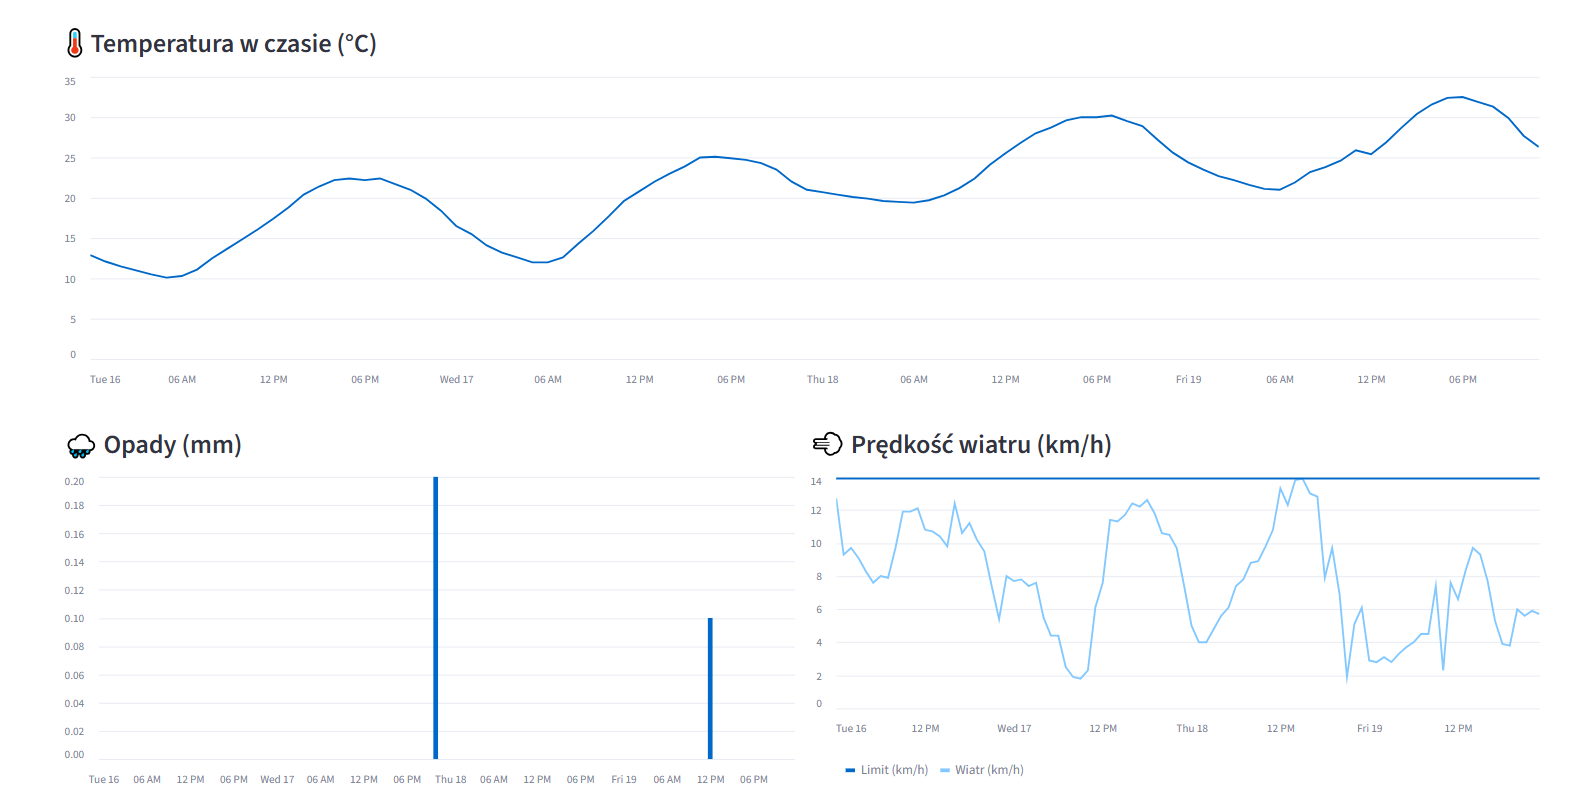
\includegraphics[width=0.95\textwidth]{img/dashboard_wykresy.png}
\captionof{figure}{Rysunek 5. Wykresy temperatury, opadów i prędkości wiatru}
\end{figure}

Sekcja jakości powietrza zawiera wykres AQI w czasie oraz wykresy PM2.5 i PM10
wyświetlane obok siebie. Widok dostępny jest zarówno w zakładce danych godzinowych,
jak i jako osobna zakładka ,,Jakość powietrza''.

\begin{figure}[H]
\centering
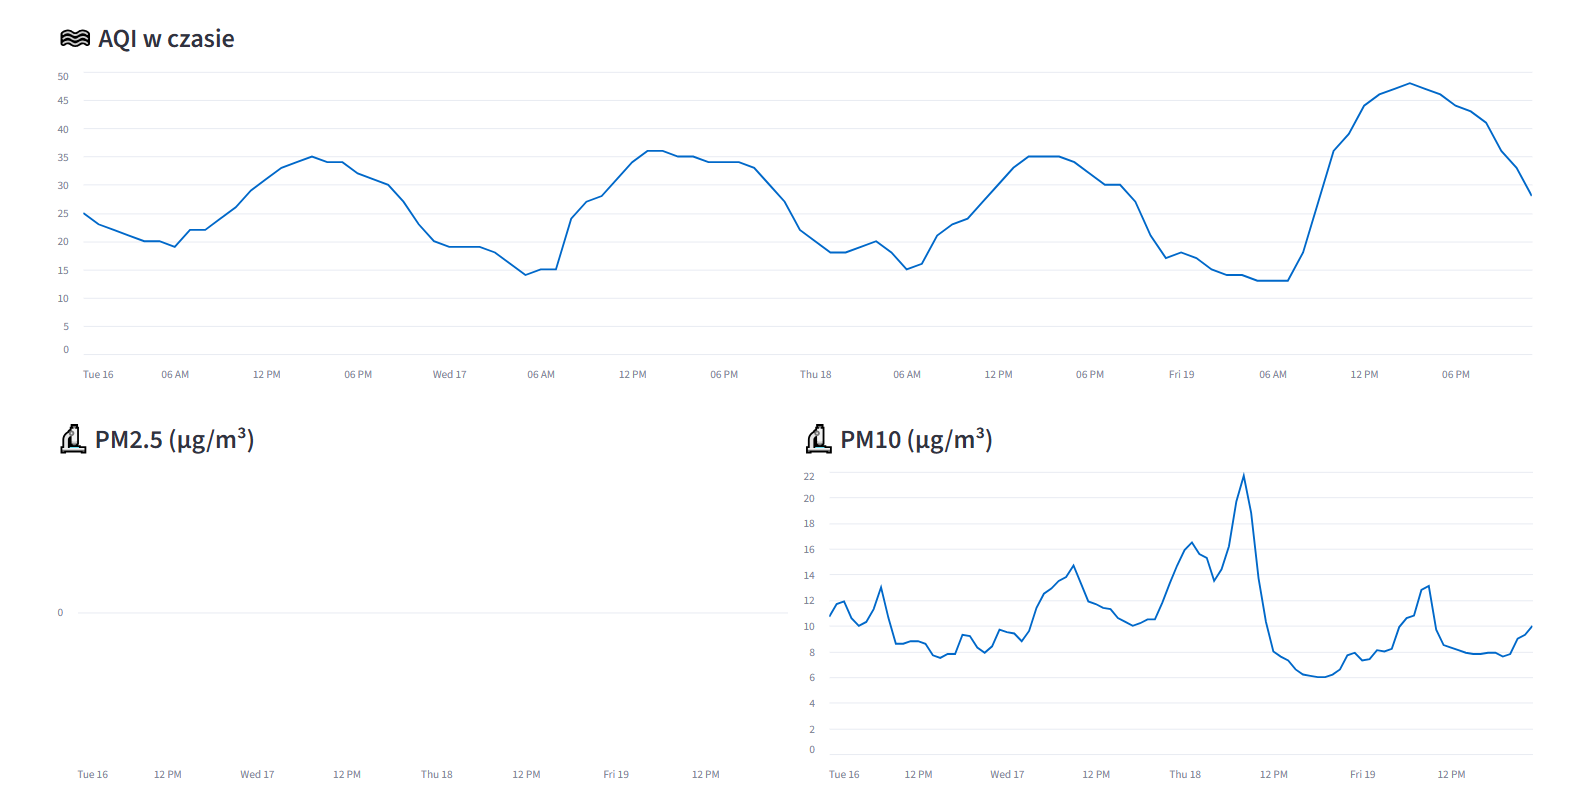
\includegraphics[width=0.95\textwidth]{img/dashboard_aqi.png}
\captionof{figure}{Rysunek 6. Wykresy jakości powietrza (AQI, PM2.5, PM10)}
\end{figure}

% ── 10. Wnioski ──────────────────────────────────────────────────────────────

\section*{\textbf{10. Wnioski}}

W ramach projektu zrealizowano kompletny system do pobierania, przechowywania
i wizualizacji danych pogodowych. Zastosowanie Open-Meteo API umożliwiło
bezpłatny dostęp do danych pogodowych i jakości powietrza w czasie rzeczywistym,
bez konieczności rejestracji ani zarządzania kluczami dostępu.

Relacyjna baza danych PostgreSQL z normalizacją przez tabelę lokalizacji
i słownik kodów pogodowych zapewniła spójność danych i czytelność wyników.
Ograniczenia \texttt{UNIQUE} i klauzula \texttt{ON CONFLICT} wyeliminowały
problem duplikatów przy cyklicznym imporcie.

Biblioteka Streamlit okazała się trafnym wyborem dla prototypu akademickiego --
umożliwiła szybkie stworzenie interaktywnego dashboardu z 12 filtrami i wieloma
typami wykresów wyłącznie w Pythonie, bez potrzeby znajomości technologii
frontendowych. Zastosowanie \texttt{@st.cache\_resource} dla połączenia z bazą
danych i parametryzowanych zapytań SQL wyeliminowało problemy z wydajnością
i bezpieczeństwem.

Projekt wykazał, że architektura oparta na automatycznym imporcie danych z API
z harmonogramem czasowym, relacyjnej bazie danych i warstwie wizualizacyjnej
jest praktycznym i łatwym w utrzymaniu rozwiązaniem dla systemów monitorowania
środowiskowego.

\end{document}
